\section{Prototypen}\label{sec:prototypen}

Prototypen werden genutzt, damit Softwarekonzepte praktisch getestet werden können.
Ihre Herstellung ist weniger aufwendig und besser adaptierbar als fertige Software.
Prototypen werden genutzt um mit Hilfe von Personas und Kontextpersonen konkrete Umsetzungsideen der Software zu testen.

Es gibt viele Varianten an Prototypen.
Im Folgenden sind die Typen "Paper Prototyp" und "Wireframe/ Mockup" genauer beleuchtet.
Es folgt eine Übersicht über weitere Prototyparten und Kriterien, mit denen ein zum Kontext passender Typ gewählt werden kann.

\subsection{Paper Prototyps}

Um einen Paper Prototyp zu erstellen, wird die überlegte Software auf Papier skizziert.
Dabei wird kein Wert auf das Design gelegt.
Wichtig sind Interaktion und Idee der Entwickelnden.
Für jede benötigte Ansicht wird ein eigener Prototyp erstellt.
Änderungen an der Oberfläche werden entweder durch einen neuen Prototypen oder zusätzliche hinzu zulegende Bausteine realisiert.
Eingabefelder können beispielsweise durch Folien mit nicht permanenten Stiften realisiert werden.

Paper Prototypen sind einfach herzustellen.
Aus diesem Grund haben Kontextpersonen eine niedrige Schwelle für Kritik und Verbesserungsvorschläge.
Diese wächst mit dem in den Prototypen investierten Aufwand.
Ebenso sind keine technischen Kenntnisse nötig, um Paper Prototypen zu erstellen.
Nutzende können im Zuge von Usability Tests direkt an ihnen mitarbeiten und ihre Kritik grafisch darstellen.

Auf Grund der niedrigen Änderungsschwelle für Paper Prototypen kann der iterative Verbesserungsprozess der Paper Prototypen jedoch in die Länge gezogen werden.
Ebenso fällt die Unterscheidung zwischen "must-haves" und "nice-to-haves" schwerer.

\subsection{Wireframes und Mockups}

Wireframes sind als digitale Paper Prototyps zu verstehen. Auch hier liegt der Fokus auf Idee und Interaktion, nicht auf Design.
Im Gegensatz zu Paper Prototyps ist die Kritikschwelle hier jedoch höher, da digitale Zeichnungen steht eine längere Entwicklungszeit suggerieren.
Dies muss im Falle von Wireframes jedoch nicht der Fall sein.
Wireframes sind statische Ausschnitte aus der zu erstellenden Software.
Ebenso wie bei Paper Prototyps werden Änderungen an der Oberfläche durch neue Wireframes dargestellt.

Aufbauend auf Wireframes existiert das Konzept von Mockups.
Unter Mockups sind Wireframes zu verstehen, welche jedoch nun auch im Thema Design ausgearbeitet sind.
Es handelt es sich hier also bereits um eine statische Version des Endproduktes.

\subsection{Weitere}

Neben den bereits benannten Prototypen gibt es eine Vielzahl weiterer Möglichkeiten der Prototypisierung.
Einige von ihnen sind \autoref{fig:prototypenUebesicht} zu entnehmen.
In der Grafik sind die Typen bezüglich den Aspekten Information, Interaktion, visuellem Design, Redaktioneller Inhalte, Branding und System bewertet.

\begin{figure}[htp]
    \centering
    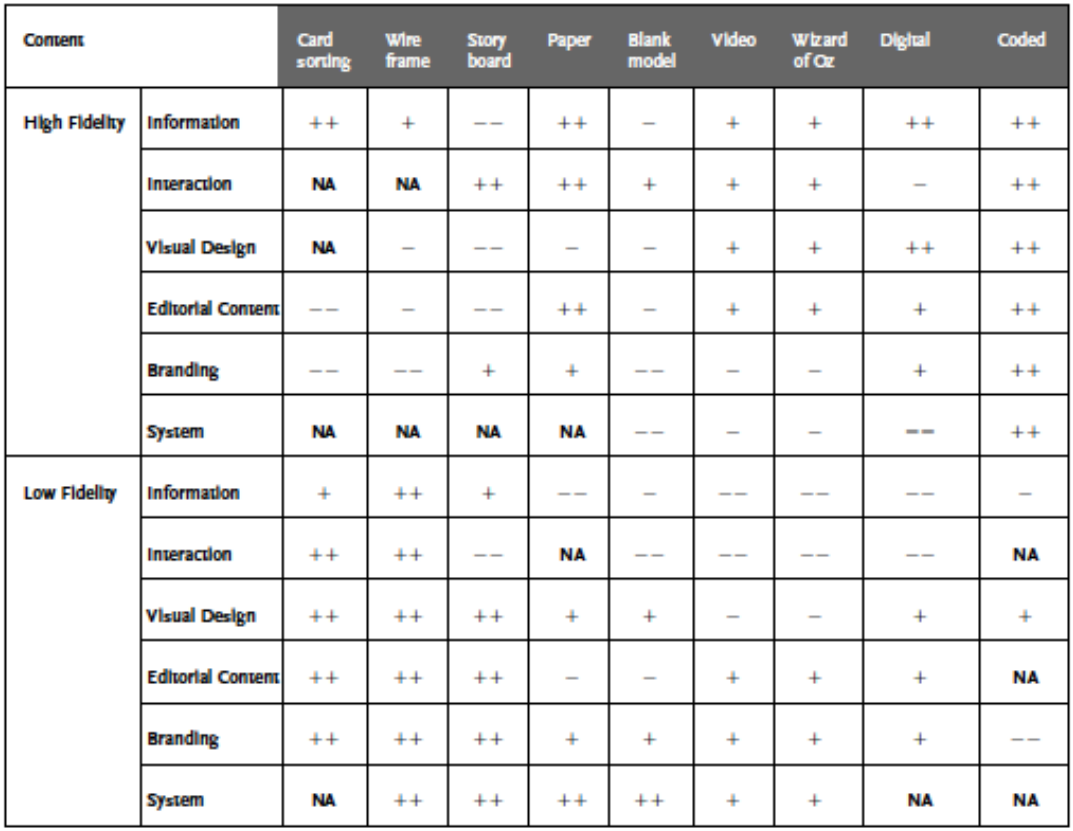
\includegraphics[width=\textwidth]{images/prototypen-übersicht.png}
    \caption{Übersicht Prototypen aus \cite{NOG}}
    \label{fig:prototypenUebesicht}
\end{figure}

Je nach Phase der Entwicklung sowie vorliegendem Kontext kann somit eine passende Art an Prototyp gefunden werden.
Die Wahl des Prototyps ist nicht auf einen einzigen beschränkt.
Mischformen oder die Verwendung mehrerer Prototypen zur selben Zeit ist möglich und in vielen Fällen auf Grund einer besseren Darstellung des Konzepts empfehlenswert.